%%
%% licence       kaneton licence
%%
%% project       kaneton
%%
%% file          /home/mycure/kaneton/view/papers/assignments/k1.tex
%%
%% created       matthieu bucchianeri   [tue feb  7 11:49:38 2006]
%% updated       julien quintard   [fri mar  3 16:31:17 2006]
%%

%
% k1
%

\section{k1}

%
% informations
%

\subsection{Informations}

\begin{tabular}{p{7cm}l}
Deadline: & XXX, 23h42 \\
Duration: & Two weeks \\
File name: & k1.tar.gz \\
In charge of: & Julien Quintard - \small{quinta\_j@epita.fr} \\
Newsgroups: & epita.cours.kaneton \\
Languages: & Assembly and C \\
Architectures: & Intel Architecture 32-bit \\
Students per group: & Three \\
\end{tabular}

%
% overview
%

\subsection{Overview}

The \textbf{k1} project consists in the development of the bootloader.

In kaneton, one of the bootloader's role is to prepare a correct
execution context for the kernel.

To do so, the bootloader has to install the proper memory addressing model
the kernel is expecting, depending on the architecture. In fact, the
kaneton microkernel assumes it is running on a microprocessor architecture
with virtual memory enabled.

Therefore, the architecture dependent source code has to deal with that,
providing kind of virtual memory so the kaneton microkernel can be executed.

Let's take some examples; for the \textit{ia32-virtual} architecture,
the booloader will install the virtual memory using microprocessor's
facilities while for the \textit{ia32-segment} architecture, the booloader
and the entire architecture dependent source code will emulate this
virtual memory using microprocessor's segmentation facilities in a very
specific way.

Another bootloader's role is to provide the kernel enough information
on the current microprocessor's architecture.

To do so, the bootloader has to fill in an initialization structure which
will be passed to the kernel at its boot time.

This structure will inform the kernel of the location of some
fundamental objects like the kernel code, the kernel stack, the initialization
structure, the modules, the segments, the regions and the alloc survival area.

We will now detail some of these components:

\subsubsection{Modules}

We call \textbf{module} any additionnal file passed at the boot time.

A module can be a picture, a binary object, a configuration file
or anything else.

Do not consider a module in the other kernels terms. A kaneton module
can be anything while the term \textit{module} is generally used to describe
a kernel module, a dynamic part of code which can be attached to the
running kernel.

In kaneton, modules are used to pass the kaneton configuration file
which contains the kaneton parameters and describes the kaneton servers
to launch as soon as possible. The kaneton servers' binary objects to
launch are also passed as modules.

Of course the bootstrap has to handle kind of modules, otherwise it will
not be capable of passing them to the bootloader.

The bootloader must build a special data structure containing everything
necessary to get access to the modules including: number of modules,
modules' information, modules' content etc..

In fact, the kernel itself will not use the modules. Indeed, a dedicated
server will be launched by the kernel and will get access to the modules.
Then this dedicated server will launch the very first servers.

To do so, the kernel will first launch this dedicated server and then
will explicitly give the area containing the modules to this dedicated
server.

It is obviously simpler to give one area containing the modules
stuff rather than giving an area containing the modules information, then
an area per module and finally another area containing the modules' string
names.

For these reasons, a very specific area must be built to contain
to whole stuff in relation with the modules so the kernel just has to
give this area to the dedicated server.

The modules area has the following form:

\begin{enumerate}
  \item
    A \textit{t\_modules} structure specifying some general information on
    the modules like the number of modules.
  \item
    An array of variable length modules, each module being composed of:

    \begin{enumerate}
      \item
	A descriptor \textit{t\_module} containing the module's size and
	a pointer to the module's name.
      \item
	The module content.
      \item
	The module's string name terminated by a zero character.
    \end{enumerate}
\end{enumerate}

Be careful, the array of modules is a variable length item array.
Module data and name are variable length blocks.

The dedicated server will refer to the module descriptors to browse
throught the modules.

The calculation used to compute the next module address is:

\begin{verbatim}
sizeof(t_module) + module->size + strlen(module->name) + 1
\end{verbatim}

A smart idea would be to add a \textit{next} field in the \textit{t\_module}
structure to directly go through the next module. Obviously we could
add another interesting field: \textit{content} referencing the module's data.

\subsubsection{Segments}

A \textbf{segment} is simply a contiguous area of used physical memory.

We introduced the term for nomenclature reasons.

Notice that a segment in the kaneton terms has nothing to do with
a segment in some architectures terms.

In fact, the kaneton kernel has to provide physical memory operations to
reserve, release physical memory areas or segments. To do so, the kaneton
core is composed of a \textbf{segment manager} which provides an interface
to manipulate the segments.

As an example, let's consider the segment reservation which is a very
common segment operation. This operation looks for a contiguous area
of unused physical memory in its internal data structure and then
returns an identifier on this area.

Now, consider that, at the kernel boot time, the segment manager has
an empty data structure. Then the segment manager can choose any
unused area and return an identifier on it. \textit{any unused area} means
any unused physical memory area including the kernel code area, the kernel
stack area, the modules area, the architecture dependent areas like maybe the
video memory area and the BIOS mapping area etc..

You should understand that the kaneton core needs to know which physical
memory area should not be reserved or are pre-reserved.

So, the bootloader must build a data structure containing the set of
pre-reserved segments. By pre-reserved segments we mean every fundamental
and distinctive areas.

This data structure will be used by the task manager to properly
initialize the kernel's address space used by the kernel task object.

In other words, the segment array describe the initial state of the
segment manager, so the initial state of the physical memory hold by the
kernel.

Therefore it will be impossible, for example, to reserve an area
already hold for something else.

Then, once the segment manager is initiliazed, the segments are reserved
and released as usual. So, every segment which become useless has to be
released.

\subsubsection{Regions}

A \textbf{region} is a contiguous area of used virtual memory.

A region maps a segment part, or the whole.

The region array describes the initial state of the region manager, or
the initial kernel's virtual memory state.

The kernel's task manager will so go through this data structure
and properly rebuild the virtual memory from this data structure to
initialize the kernel's address space.

Then, in the common case, every useless region must be released as the
segments are.

\subsubsection{Survival Area}

Like every program, kernels need memory to build and maintain internal
data structures. These data structures can be used to keep track of
the alive processes but also to keep track of the memory state.

For example, kernels typically have a kind of manager which keeps track
of the physical memory state. This manager internally uses a data
structure to know which memory areas are for example unused.

During operating systems history, different data structures were used for
this purpose from the most basic one; the bitmap which just tells whether
a physical memory page is used or not; to more complex one like the buddy
system.

Let's consider a relatively simple data structure which only keeps track
of used physical memory area in a linked-list. Each element of the
linked-list provides enough information to describe a used physical memory
area inluding the base address, the area size, the permissions etc..

Note that, in kaneton terms, this manager is called the segment manager.

Therefore, to maintain such a data structure this manager needs memory.
Nevertheless, it seems impossible since this manager is actually initializing
its internal data structure to provide this functionality.

You can notice that this manager needs memory while it is its role to provide
an interface to allocate memory.

This mutual dependency generally leads to static and specific implementations.

Indeed, kernels usually use a very specific data structure to install
the physical memory manager. Then the other parts of the kernels can allocate
memory without taking care of anything.

But the price to pay is to, for example, implement a simple static array
which will be linked with another one when the elements to manage become
too important.

Then, the kernels' physical memory managers are typically ugly for this
precise reason.

We wanted kaneton to be elegant in every points. So we had to choose another
solution to this typical problem to permit kaneton to evolve in a very
coherent way where everything is dynamic and based on other kaneton
managers.

In kaneton, the data structures are managed by the set manager. This
manager uses the malloc() function to allocate fine-grained memory.
This set manager is used by every kaneton manager to store data.

Now let's come back to our physical memory manager problem. Recall that, in
kaneton, the physical memory manager is the segment manager.

We wanted to build the segment manager over the set manager so the segment
manager can use dynamic data structures and not ad-hoc data structure
solutions.

The segment manager uses the set manager which is based on the
malloc() function. Then the malloc() function needs to allocate
physical memory areas to provide fine-grained allocation in them. Once
again, there is an evil mutual dependency between malloc() and the segment
manager.

To break this mutual dependency we decided to give the malloc() function
a pre-reserved area so it can use it to provide fine-grained memory until
the segment and region managers are initialized.

Once the segment and region managers will be initialized, the malloc()
function will just have to reserve physical memory to perform the same
work than every typical malloc() function do.

Since, at the core boot time, the segment manager is not initialized yet,
the core itself cannot decide where to put this pre-reserved area.

Therefore, the kernel relies on the bootloader to find out a pre-reserved
area of physical memory for the malloc() function. This area will then
be called the \textbf{survival area} or someties the
\textbf{survival segment}.

\subsubsection{Initialization Structure}

As mentioned before, the bootloader has to build an initialization structure
and to pass it to the kernel so the kernel can locate the different
fundamental objects in memory.

The initialization structure called \textbf{t\_init} is defined in the
file \textit{core/include/kaneton/init.h}.

We will now detail the fundamental fields:

\begin{itemize}
  \item
    \textbf{mem} and \textbf{memsz} indicate the computer's available
    physical memory.
  \item
    \textbf{kcode} and \textbf{kcodesz} indicate the location and
    size of the kernel binary object in main memory, after relocation.
  \item
    \textbf{init} and \textbf{initsz} fields indicate the location and
    size of this initialization structure in main memory.
  \item
    \textbf{modules} and \textbf{modulessz} indicate the location of
    the area used to store the modules.
  \item
    \textbf{nsegments}, \textbf{segments} and \textbf{segmentssz}
    indicate the area location containing the segment array. This
    array describes the core's pre-reserved segments.

---
    For the bootloader, the only required fields of the \textit{o\_segment}
    structures are \textit{segid}, \textit{address}, \textit{size} and
    \textit{perms}.

    Other fields will be filled in at kernel initialization time.

    Note that the \textit{segid} field must be equal to the
    \textit{address} one.
---

  \item
    \textbf{nregions}, \textbf{regions} and \textbf{regionssz} fields
    indicate the area location containing the region array. This array
    describes the segments to be mapped after the initialization of the
    core region manager.

---
    The bootloader must fill in the \textit{segid}, \textit{address},
    \textit{offset} and \textit{size} fields of each \textit{o\_region}
    structure.

    Since many segments will be needless, this array will only specify the
    fundamental segments to map.
---
  \item
    \textbf{kstack} and \textbf{kstacksz} indicate the kernel stack
    area location.
  \item
    \textbf{alloc} and \textbf{allocsz} fields indicate the location
    and size of the fine-grain allocator survival area.

    This area will be used by the malloc() function to provide fine-grain
    allocator while no segment neither region manager are initialized
    yet.

    The bootloader may allocate about sixteen pages for the survival area.
\end{itemize}

The initialization structure also contains machine-dependent fields.

Look at the file \textit{core/include/arch/[architecture]/kaneton/init.h}
for more information about the structure machine-dependent initialization
structure called \textbf{d\_init}.

%
% assignments
%

\subsection{Assignments}

In this project, the students have to develop the entire source code.
This means that no interface will be provided.

The only requirement is your bootloader to be compliant with the
initialization structure passed to the kaneton microkernel.

If this structure is not correctly built, then the kernel would not
be able to run.

Below are listed the bootloader's steps:

\begin{enumerate}
  \item
    The bootloader generally installs a more evolved memory addressing model,
    depending on the architecture.
  \item
    The bootloader relocates the stuffs needed by the future kernel
    execution and build the initialization structure.

    The stuff includes:

    \begin{itemize}
      \item
	The kernel code.
      \item
	The modules.
      \item
	The pre-reserved segments.
      \item
	The pre-reserved regions.
      \item
	The kernel stack.
      \item
	The alloc survival area.
    \end{itemize}
  \item
    Then, the booloader prepares the kernel stack and calls it providing
    to the kernel a complete initialization structure.
\end{enumerate}

The relocation is not really necessary but we wanted the students
to understand low-level programming and more especially programming
in a very strict environment with no fine-grain allocator provided.

The main goal of this project is to lead the students to understand the
project source organization. Indeed, a complete development environment
is provided; therefore, the students should learn to use system defines,
internal facilities etc.. to develop more quickly.

Displaying the initialization structure's information is the
minimum requirement. Having an enhanced display of pre-reserved
segments, regions and modules will be very appreciated, but is not required.

The code provided must be located in the directory
\textit{core/bootloader/arch/[architecture]/}.

\subsubsection{Tips}

Try to think about a very simple memory allocator delivering single
pages or contiguous areas. This allocator should help students to
allocate dynamic memory.

Assume that the kernel is the first given module.

\subsubsection{Additional Work}

Moreover, students should write a tiny console driver. Try to make this
driver code generic so you can reuse it in the next steps.

Finally, for this project, the students have to initialize the segment
and region manager, based on the segment and region array provided by
the bootloader's initialization structure. Note that this specific
initialization will change in the next projects.

\subsubsection{Bonus}

Be creative...

%
% ia32
%

\subsection{Intel Architecture 32-bit Implementation}

The bootloader is highly specific to the architecture because its main
roles are to:

\begin{itemize}
  \item
    Install new memory addressing models.
  \item
    Build the pre-reserved segment array.
  \item
    Build the pre-reserved region array.
\end{itemize}

The other tasks are independent of the architecture.

We will so detail the three previous points.

\subsubsection{Memory Addressing Models}

Since the kaneton microkernel can be implemented for three sub-architectures,
different Intel memory addressing models can be used.

We will assume in this document that the students implementing the
Intel architecture are using the \textit{ia32-virtual} architecture, meaning
that they are implementing the kaneton microkernel with true virtual memory.

Students willing implement kaneton with other specific Intel architecture
facilities should be able to adapt the assignments to their case.

So, in the case of the \textit{ia32-virtual} architecture, the bootloader
has to install two memory addressing models:

\begin{enumerate}
  \item
    First, the protected mode even if the bootstrap maybe installed it
    before.

    Indeed, the bootloader needs to rebuild the protected mode to be sure
    it is installed and to be able to maintain it.
  \item
    Then, the paging mode to enable virtual memory.
\end{enumerate}

We advise you to install the protected mode, then to relocate the stuff
and build the initialization structure and finally to install the
virtual memory before calling the kernel.

In this way, you will handle the hardest architecture problem, the virtual
memory, at the end, before performing the very last step, call the kernel.

\subsubsection{Segments}

The segment array passed to the kernel by the bootloader to the kernel via
the initialization structure is used to describe architecture dependent
physical memory areas as kaneton memory areas.

The kaneton memory areas are the logical memory areas to keep from being
erased like the kernel code, the kernel stack, the initialization structure,
the modules, the segment and region arrays, the survival area etc..

These areas, the core might be able to find out by itself but we prefer
specifying them in the segment array so everything is clear.

The architecture dependent memory areas are physical memory areas that
have a very special meaning on the running architecture. These area can
include the mapped video memory, the mapped BIOS ROM etc..

To keep the core segment manager from allocating memory on them, the
bootloader has to describe these areas via the segment array.

So the architecture dependent segments should include the ISA memory segment
and any other architecture specific reserved memory area for example for
the virtual memory page directories and page tables etc..

\subsubsection{Regions}

The region array must describe the virtual memory state on the specific
architecture for the kernel address space.

In other words, the region array must contains every virtual memory
areas in use once the region manager is initialized.

So, on the Intel architectures these include the mapped video memory,
the kernel code, the kernel stack, the initialization structure, the
survival area and any additional Intel specific objects like the Global
Descriptor Table etc..

Notice that it might be smart not to include the first memory page in
the region array. Mapping this page will cause null pointers to be valid!

\subsubsection{Example}

Below is a sample physical memory layout for the Intel architectures:

\begin{center}
  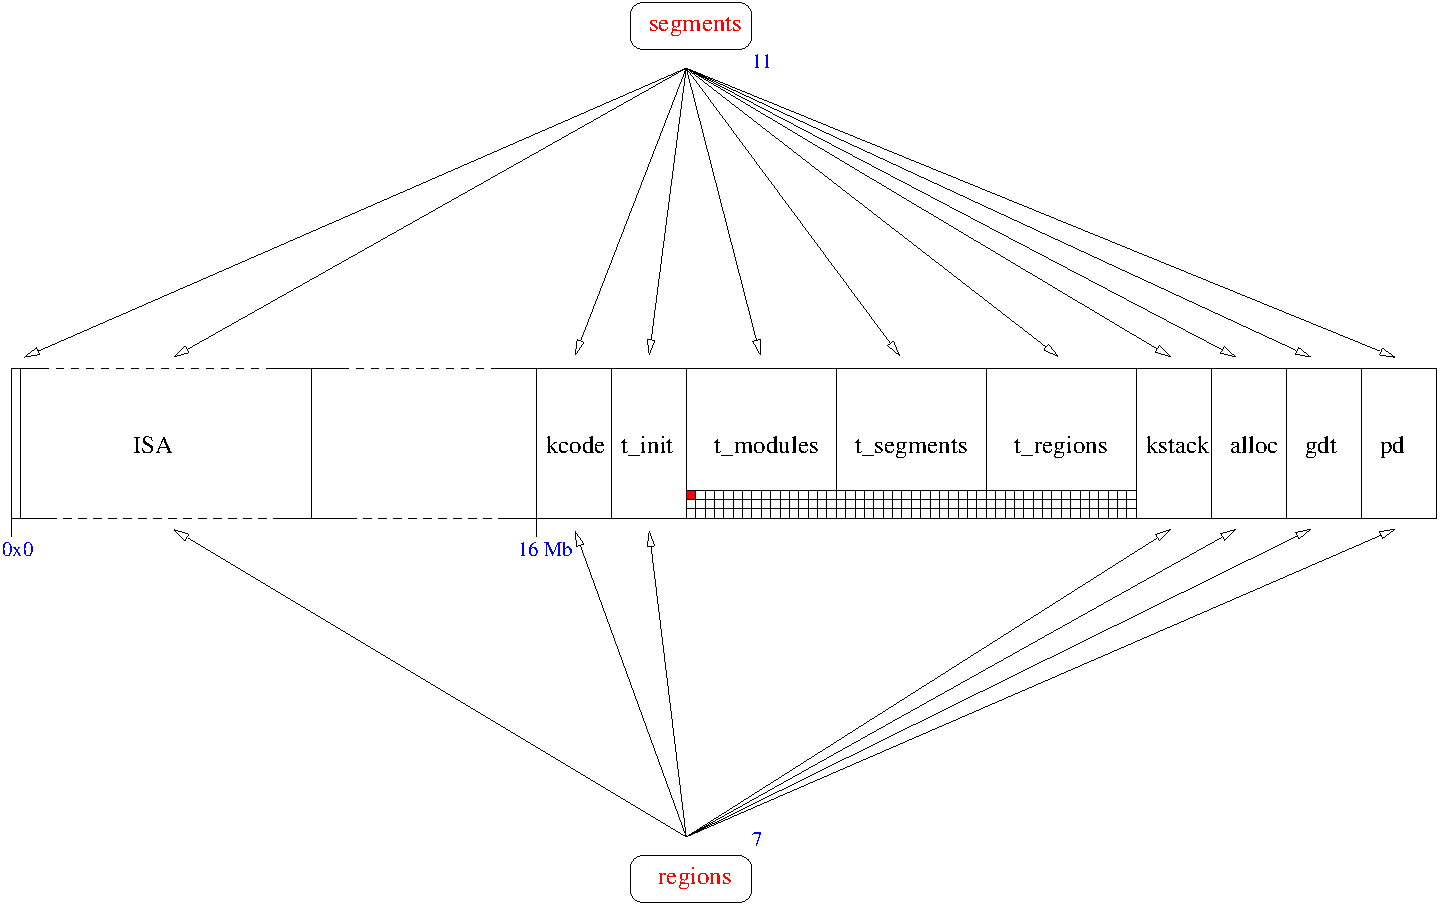
\includegraphics[scale=0.7]{figures/k1-memory-layout.pdf}
\end{center}
